\section{Описание решения} \label{label-description}
\subsection{Первая версия FlatArray}
Раскладка полей внутри FlatArray изображена на \ref{first-fa}.
Данная структура состоит из нескольких частей:
\begin{enumerate}
	\item header; заголовок объекта, который включает в себя markWord, поля для хранения длины массива и KID элемента.
	\item последовательность ссылок на объекты
	\item сами объекты
\end{enumerate}
\begin{figure}[h]
	\caption{Первая версия FlatArray}\label{first-fa}
	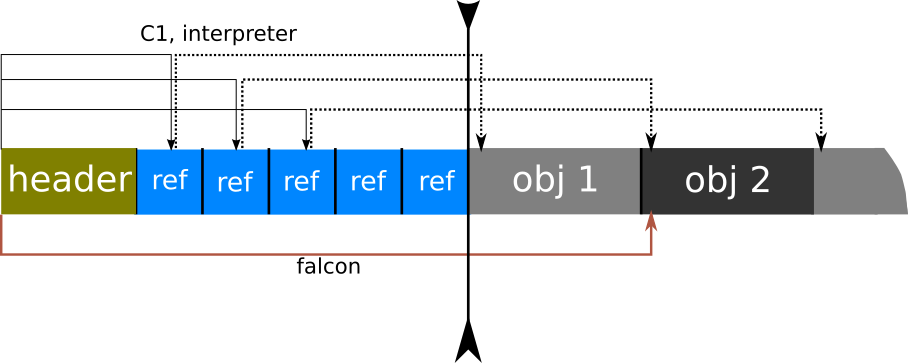
\includegraphics[width=0.95\linewidth]{image/flatarray.png}
\end{figure}
В реальности этот FlatArray представляет собой обычный Java массив класса Type[].class, у которого позади расположены элементы. Доступ к определенному элементу может быть осуществлен двумя способами: стандартным, через чтение и разыменование указателя, или путем вычисления адреса. 
JVM использует оба подхода. При интерпретации или исполнении С1 скомпилированного кода применяется первый подход, falcon - второй. 
Как упоминалось ранее, режим С1 и интерпретатор используют JNI методы для работы с FA. Однако при falcon компиляции JNI реализации подменяются специально подготовленными интринсиками. 
Свойство nullability достигается путем добавления поля 'isSentinel' во внутрь элемента. 
В конечном итоге такая раскладка FlatArray имеет ряд недостатков:
\begin{enumerate}
	\item Проверка nullability достаточно медленная. Особенно в случае not-existing, поскольку мы имеем большее число промахов кеша по сравнению с классическим Java массивом.
	\item Необходимо вычислять размер элемента массива для адресной арифметики, что дает значительные накладные расходы. Либо необходимо хранить размер элемента где-то внутри структуры данных, что и было применено в последствии.
	\item Нет поддержки сборки мусора, поскольку такой FlatArray неотличим от обычного Java массива объектов. 
	Необходимо корректно предоставлять метаинформацию о этом объекте. 
\end{enumerate}

\subsection{Представление FlatArray с sentinel array}
В этом разделе представлена альтернативная версия раскладки полей FlatArray. В ней учтены недостатки предыдущего подхода.
\begin{figure}[h]
	\caption{Первая версия FlatArray}\label{first-fa}
	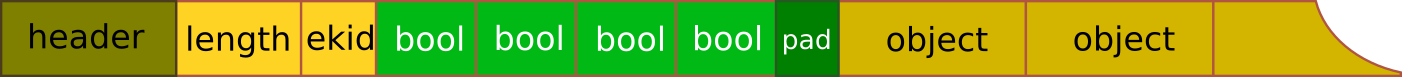
\includegraphics[width=0.95\linewidth]{image/flatarray-new.png}
\end{figure}
Этот массив состоит из следующих полей:
\begin{itemize}
	\item header[8 byte]; markWord этого объекта
	\item length [4 byte]; длина массива
	\item ekid [4 byte]; KID элемента массива
	\item sentinel array; массив элементов типа bool, который показывает, какие элементы внутри были явно инициализированы
	\item pad; поле для выравнивания 
	\item Последовательность элементов вместе с метаинформацией
\end{itemize}
Поля 'isSentinel' вынесены в одну компактную область памяти, что в итоге уменьшает число промахов кеша в режиме 'not-existing'.
Результаты тестирования производительности можно увидеть в таблицах \ref{sentinel-hashMap-perf1}, \ref{sentinel-hashMap-perf2} и \ref{sentinel-hashMap-perf3}. Описание тестов можно найти в разделе \ref{benchmarks}.

\begin{table}[H]
	\centering
	\caption{Производительность HashMap only-existing.}\label{sentinel-hashMap-perf1}
	\textit{\begin{tabular}{|c|c|}
			\hline Benchmark  & Score, op/s \\
			\hline faMapLoop  & 5523 \textcolor{red}{-2\%} \\
			\hline mapLoop    & 5646 \\
			\hline 
	\end{tabular}}
\end{table}

\begin{table}[H]
	\centering
	\caption{Производительность HashMap fifty-fifty.}\label{sentinel-hashMap-perf2}
	\textit{\begin{tabular}{|c|c|}
			\hline Benchmark  & Score, op/s \\
			\hline faMapLoop  & 6122 \textcolor{green}{+5\%} \\
			\hline mapLoop    & 5833 \\
			\hline 
	\end{tabular}}
\end{table}

\begin{table}[H]
	\centering
	\caption{Производительность HashMap not-existing.}\label{sentinel-hashMap-perf3}
	\textit{\begin{tabular}{|c|c|}
			\hline Benchmark  & Score, op/s \\
			\hline faMapLoop  & 34216 \textcolor{green}{+12\%} \\
			\hline mapLoop    & 30371 \\
			\hline 
	\end{tabular}}
\end{table}

\subsection{Текущее представление FlatArray}
Новое внутреннее представление FlatArray изображено на рисунке \ref{last-fa}
\begin{figure}[h]
	\caption{Текущее представление FlatArray}\label{last-fa}
	
\includegraphics[width=0.95\linewidth]{image/flat-array-without-sentinel.png}
\end{figure}
Этот массив имеет несколько полей:
\begin{itemize}
	\item markWord [8 byte]; 
	\item length [4 byte]; длина массива
	\item ekid [4 byte]; KID элемента массива
	\item Последовательность элементов вместе с метаинформацией:
	\begin{itemize}
		\item offset[4 byte]; Смещение от заголовка текущего элемента до заголовка FlatArray.
		\item bool[1 byte]; показывает, что данный элемент был инициализирован.
		\item pad; выравнивание.
		\item object; элемент массива.
	\end{itemize}
\end{itemize}
Результаты тестирования производительности можно увидеть в таблицах \ref{new-hashMap-perf1}, \ref{new-hashMap-perf2} и \ref{new-hashMap-perf3}. Описание тестов можно найти в разделе \ref{benchmarks}.
\begin{table}[H]
	\centering
	\caption{Производительность HashMap only-existing.}\label{new-hashMap-perf1}
	\textit{\begin{tabular}{|c|c|}
			\hline Benchmark  & Score, op/s \\
			\hline faMapLoop  & 6032 \textcolor{green}{+7\%}\\
			\hline mapLoop    & 5654 \\
			\hline 
	\end{tabular}}
\end{table}

\begin{table}[H]
	\centering
	\caption{Производительность HashMap fifty-fifty.}\label{new-hashMap-perf2}
	\textit{\begin{tabular}{|c|c|}
			\hline Benchmark  & Score, op/s \\
			\hline faMapLoop  & 5393 \textcolor{red}{-7\%} \\
			\hline mapLoop    & 5824 \\
			\hline 
	\end{tabular}}
\end{table}

\begin{table}[H]
	\centering
	\caption{Производительность HashMap not-existing.}\label{new-hashMap-perf3}
	\textit{\begin{tabular}{|c|c|}
			\hline Benchmark  & Score, op/s \\
			\hline faMapLoop  & 19401 \textcolor{red}{-25\%} \\
			\hline mapLoop    & 25757 \\
			\hline 
	\end{tabular}}
\end{table}
Как видно из таблиц, поиск существующего ключа в хеш-таблице, базирующейся на FlatArray, менее эффективно, чем в стандартной HashMap, однако в других случаях мы имеем хорошую производительность.
\begin{table}[H]
	\centering
	\caption{Производительность FlatArray only-existing.}\label{new-flatArray-perf1}
	\textit{\begin{tabular}{|c|c|}
			\hline Benchmark              & Score, op/s \\
			\hline flatArrayLoop          & 58843 \textcolor{green}{+77\%} \\
			\hline basicArrayLoop         & 33184 \\
			\hline
			\hline flatArrayLoopSentinel  & 41450 \textcolor{green}{+35\%} \\
			\hline basicArrayLoopSentinel & 30810 \\
			\hline
			\hline flatArray              & 653577811 \textcolor{green}{+13\%} \\
			\hline basicArray             & 579119776 \\
			\hline
			\hline flatArraySentinel      & 387515918 \textcolor{green}{+4\%} \\
			\hline basicArraySentinel     & 373422833 \\
			\hline 
	\end{tabular}}
\end{table}

Результаты тестирования производительности элементарных операций над FlatArray и Java массивом объектов приведены в таблице \ref{new-flatArray-perf1}. Как мы видим, FlatArray имеет лучшие результаты, чем обычный массив.
\par
После анализа было выяснено, что является главной причиной, почему производительность FlatArray в HashMap не дает похожего улучшения. Это связано с тем, что в HashMap чтение памяти не является узким местом, то есть производительность поиска по ключу ограничена пропускной способностью процессора, а не памяти. Связи с этим, FlatArray будет полезен в тех местах, где бутылочным горлышком будет доступ к памяти.

\subsection{Методика тестирования производительности FlatArray} \label{benchmarks}
\subsubsection{Особенности тестирования производительности кода в JVM языках}
Поскольку целью данной работы это оптимизация производительности, то важной задачей становится подбор подходящих метрик для ее измерения. FlatArray новая структура данных для Java мира и готовых бенчмарков для ее тестирования не существовало. 
В результате данной работы была создана коллекция тестов, которые измеряют производительность FlatArray по сравнению с обычным Java массивом с учетом различных аспектов.
В частности, тесты измеряют скорость доступа к элементу массиву в зависимости от его длины. Так же учитываются такие факторы, как nullability элемента. Измерение скорости доступа проводится в трех режимах:
\begin{enumerate}
	\item not-existing; структуре данных полностью пуста
	\item fifty-fifty; структура данных на 50\% пуста
	\item only-existing; полная инициализация всех элементов
\end{enumerate}
Помимо сравнения массивов, были созданы тесты, измеряющие производительность HashMap из JDK8 и хеш-таблицы, основанной на FlatArray. Эти бенчмарки позволяют оценить потенциальную применимость данной структуры данных внутри JDK. Они измеряют производительность операции поиска по ключу в трех режимах, описанных в этом разделе.
Все измерения проводились на компьютере с процессором Intel(R) Xeon(R) E-2134 CPU @ 3.50GHz
с объемом оперативной памяти 64Gb.
\par
Как утверждалось ранее, JVM это управляемая среда исполнения с JIT компиляцией и функцией автоматической сборки мусора. Это сильно сказывается на методике измерения, поскольку JVM может выдавать нестабильную производительность. 
В первую очередь это связано с тех, что JVM достигает пиковой производительности далеко не сразу после старта приложения.
Среде исполнения необходимо время, чтобы загрузить требуемые классы, создать профиль исполнения приложения, скомпилировать горячие методы и так далее.
Процесс разгона JVM до пиковой производительности называют "warm-up", или "разогревом".
\par
Для тестирования производительности кода, написанного на JVM языках, существуют специализированные инструменты. 
В данной работе применялся Java Microbenchmark Harness\cite{jmh}. Это набор библиотек для измерения производительности небольших кусков кода.
Этот инструмент позволяет разработчику настраивать время warm-up, количество итераций измерений, а так же выбирать формат представления результатов. 
В работе используется throughput, которая выражается в количестве операций в секунду, то есть op/s. 
\par
Ниже в разделах будут описаны конкретные тесты производительности, что они измеряют и зачем. В дальнейшем в работе будут приводится результаты бенчмарков для различных версий FlatArray.

\subsubsection{Тесты flatArrayLoop и basicArrayLoop}
Эти бенчмарки тестируют производительность обхода массива в цикле. Код теста выглядит примерно так:
\begin{lstlisting}
	measure() {
		for (int i = 0; i < length; i++) {
			long value = array[indexes[i]].field;
			acc = doSimpleMath(acc, value)
		}
		return acc;
	}
\end{lstlisting}
В случае когда 'array' это FlatArray, бенчмарк носит название flatArrayLoop и basicArrayLoop, если в качестве 'array' применяется стандартный Java массив.
Тест обходит 'array' по заранее подготовленным индексам, содержащихся в 'indexes'. 
Из массива извлекается объект, из которого читается поле типа long. В дальнейшем оно используется для вычисления простой арифметики в функции 'doSimpleMath'. 
Массив 'index' предварительно заполняется индексами. При этом существует два режима обхода 'array':
\begin{enumerate}
	\item random; каждый последующий индекс это псевдослучайное число.
	\item forward; индексы идут по возрастающей от 0 до 'length'
\end{enumerate}

\subsubsection{Тесты flatArray и basicArray}
Эти тесты используются для измерения скорости одиночного доступа к полю элемента массива. Псевдокод приведен в листинге:
\begin{lstlisting}
	measure() {
		long value = array[index].field;
		return value;
	}
\end{lstlisting}
В отличие от тестов из прошлого раздела, эти тесты хорошо показывают стоимость адресной арифметики. 
Компилятор способен выносить некоторые вычисления за пределы цикла, что в итоге сказывается на полученных результатах.
В случае FlatArray важно понимать реальные накладные расходы вычисления адреса конкретного поля в зависимости от длины массива.
\subsubsection{Тесты flatArraySentinel и basicArraySentinel}
Эти тесты измеряют производительность доступа к элементу с явной проверкой на nullability. Псевдокод показан ниже:
\begin{lstlisting}
	measure() { // FlatArray
		if (array.sentinel(index)) {
			acc = array.get(index);
		}
		return acc;
	}
	measure() { // Java object array.
		Element value = array[index];
		if (value != null) {
			acc = value.field;
		}
		return acc;
	}
\end{lstlisting}
\subsubsection{Тесты flatArraySentinelLoop и basicArraySentinelLoop}
Этот набор тестов похож на предыдущий, но они работают в цикле. Ниже приведен псевдокод для версии с FlatArray и с обычным Java массивом.
\begin{lstlisting}
	measure() {
		for (int i = 0; i < array.length(); i++) {
			if (array.sentinel(indexes[i])) {
				long value = array.get(indexes[i]).field;
				acc = doSimpleMath(acc, value)
			}
		}
		return acc;
	}
\end{lstlisting}

\begin{lstlisting}
	measure() {
		for (int i = 0; i < array.length(); i++) {
			Element value = array[indexes[i]];
			if (value != null) {
				acc = doSimpleMath(acc, value.field)
			}
		}
		return acc;
	}
\end{lstlisting}

\subsubsection{Тесты faMapLoop и mapLoop}
Помимо тестов непосредственно на массивы, измерялась производительность двух реализаций java.lang.HashMap. 
Обе базируются на хеш-таблице из JDK8, но одна из них использует FlatArray. 
\par
Эта пара бенчмарков тестирует скорость поиска элемента по ключу в цикле. Их псевдокод приведен ниже.
\begin{lstlisting}
	measure() {
		for (int i = 0; i < length; i++) {
			Element value = hashmap.get(keys[i]);
			if (value != null) {
				acc = doSimpleMath(acc, value.field)
			}
		}
		return acc;
	}
\end{lstlisting}

\subsubsection{Тесты faMap и map}
Помимо тестирования производительности поиска ключей в цикле, полезно измерить скорость одиночного доступа к хеш-таблице.
\begin{lstlisting}
	measure() {
		Element value = hashmap.get(key);
		return value.field;
	}
\end{lstlisting}
Эти бенчмарки отличаются от faMapLoop и mapLoop. Было замечено, что компилятор по разному оптимизирует эти два типа тестов, а потому необходимы результаты измерений обоих. 

\clearpage